\section{Introduction}
\subsection{Previous work}
Current research started as part of the studies on the Mathematics Expert in
Data Analytics and Machine Learning postgraduate specialization program \cite{_ai&ml_}
held by the AI Research Group of Eötvös Loránd University \cite{_ai_}.
During the one year program a thesis work has to be created that is often
preceeded by a modeling practice in the first semester.
This project follows the same approach as railway track fault detection models
were already built in the first semester.
However the characteristics of the dataset used at that time did not allow a
successful application of a model however valuable experience is gained together
with a boost of motivation to follow up the topic and deepen the knowledge in the
mentioned problem.

\subsection{Available results}
The work of the first semester can be found at \cite{tomcom_mathemathical_2022}.
Following is a short summary of the results obtained.

During the first semester basic convolutional neural networks were built with a classification
head to identify images with defective railway tracks.
LeNet-5, AlexNet, VGG16 and ResNet50 were applied, partially utilizing transfer learning as well
(indicated with \lstinline{*_p} in the following Figures).

The dataset was taken from the Kaggle webpage \cite{_railway_} consisting of a limited
number of images with defective and non-defective railway tracks.
The images combine a high variety of failures with very limited examples leading to a very
specific dataset where the provided validation and test split is not representing the initial
set of images.

The results of the modeling is shown on Figure \ref{fig:Kaggle_results}, where the performance of
different bootstrapped models on the splits of the dataset is given.

\begin{figure}[!ht]
    \centering
    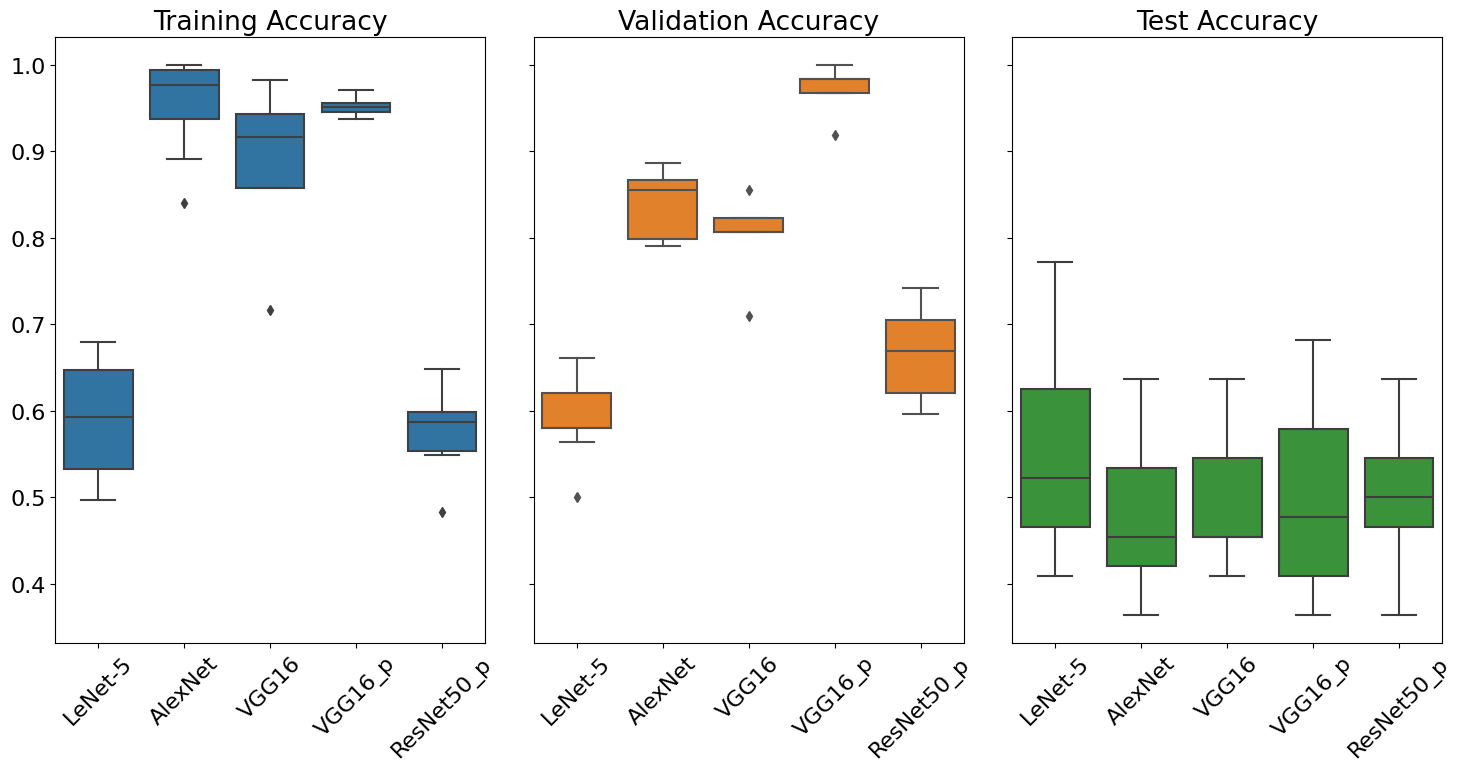
\includegraphics[width=\textwidth]{./tex_images/bootstrap_results.png}
    \caption{Results of first classification approach on the Kaggle dataset}
    \label{fig:Kaggle_results}
\end{figure}

Most of the models were successfully learned the features of the training and validation datasets,
however on the test dataset all failed to classify the images in an acceptable level, mostly
achieveing the level of a random classifier only.
This lead to the realization that the low number of images compared with the high variety of the track
failures will result in a situation where the model can easily learn the specifics of the training and
validation dataset preventing of any generalization to the test dataset.

As a followup a search for a more extended dataset and more refined models were started.

\subsection{MÁV KFV Kft.}

HISTORY!!!


The company MÁV Central Rail And Track Inspection Ltd. (MÁV KFV Kft.) \cite{_mav_} was approached
as they are proficient in railway track inspection and have the equipment and data that could be used
for building such classifier model.

Currently MÁV KFV Kft. operates two vehicles for rail inspection purposes, the SDS and FMK-008 shown on
Figure \ref{fig:vehicles}, both equipped with different measurement and inspection systems.
Fortunately both of them is equipped with video recording, however with different systems.
After a first view on the video files the system of the SDS vehicle is selected for a first modelling
approach.

\begin{figure}[!ht]
    \centering
    \begin{subfigure}{0.45\textwidth}
        \centering
        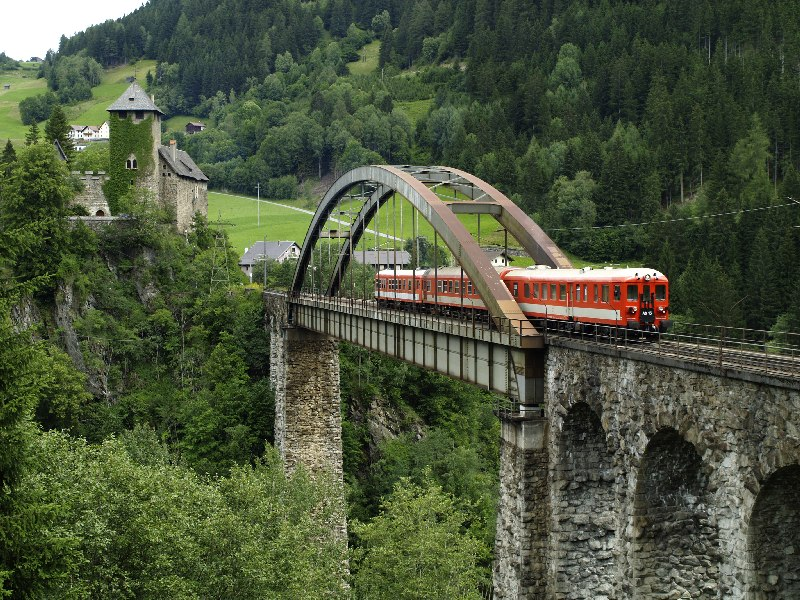
\includegraphics[height=3cm]{./tex_images/sds.jpg}
        \caption*{SDS}
    \end{subfigure}
    \begin{subfigure}{0.45\textwidth}
        \centering
        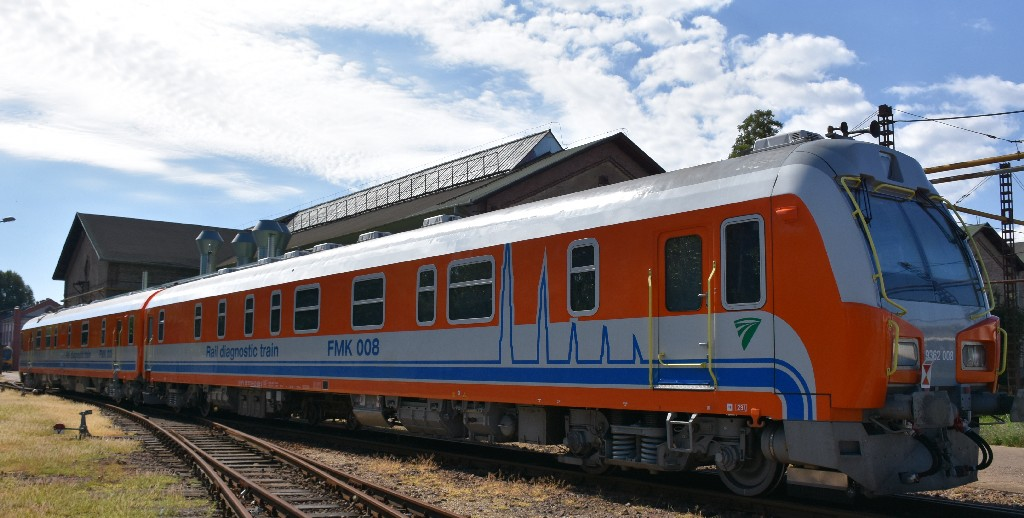
\includegraphics[height=3cm]{./tex_images/FMK008.jpg}
        \caption*{FMK-008}
    \end{subfigure}
    \caption{Railway inspection vehicles of MÁV KFV Kft.}
    \label{fig:vehicles}
\end{figure}